%%% Local Variables:
%%% mode: latex
%%% TeX-master: "../index"
%%% End:

% Recommended:
% Show symmetric-key example with Alice-Bob diagram
% Mention modern algorithm (e.g. AES, Triple-DES)
% Benefits of public-key encryption (no key sharing)
% Show public-key example with RSA and Alice-Bob diagram
\subsection{Agenda}
\begin{enumerate}
\item Symmetric-key encryption
\item Symmetric- vs. public-key encryption
\item RSA
\end{enumerate}
\subsection{Symmetric-key encryption}
\subsubsection{Set up}
\begin{itemize}
  \item $m \in \mathcal{P}$ is the plaintext
  \item $k \in \mathcal{K}$ is the key
  \item $c \in \mathcal{C}$ is the ciphertext
  \item $e_k(m)$ encryption function
  \item $d_k(c)$ decryption function
\end{itemize}

\begin{figure}[H]
  \begin{centering}
    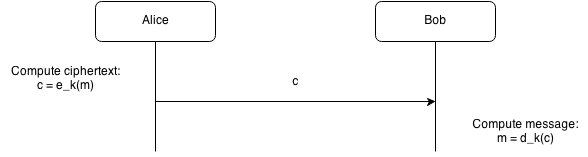
\includegraphics[width=15cm]{images/1-sym-enc}
    \caption{Basic model for symmetric encryption}
  \end{centering}
  \label{fig:sym-enc}
\end{figure}

\subsubsection{Modern implementations}
\begin{description}
\item[DES] 64-bit block cipher with 56-bit key. Due to small key,
  exhaustive search is a possibility. Therefore, \emph{Triple-DES} was
  made.
\item[AES] 128-bit block cipher with 128 to 256-bit key.
\end{description}

\subsection{Symmetric- vs. public-key encryption}
\begin{description}
\item[Pros] Faster and easier to implement
\item[Cons] Requires both parties can access the secret key. Impossible?
\end{description}

\subsection*{RSA}
\begin{itemize}
\item Public key = $(n,e)$
\item Private key = $(p,q,d)$ where $ed \equiv 1 \mod \phi(n)$.
\item Encryption is done by $Enc(m)= m^e \mod n$.
\item Decryption is done by $Dec(c)=c^d \mod n$.
\item $n = pq$, where $p$ and $q$ are odd primes (big primes makes encryption safer)
\item $e \in \mathbb{Z}^*_{\phi (n)}$, where $\phi (n)=(p-1)(q-1)$
\item $d$ is the multiplicative inverse of $e \mod \phi(n)$
\end{itemize}

\subsubsection{Weakness}
\begin{itemize}
\item Attacker can get factors of $n$
\begin{itemize}
\item If attacker can factor $n$ then he can find $d$ same way that
  the system computes it
\end{itemize}
\item Attacker finds $\phi (n)$, then factors $n$
\begin{itemize}
\item If $n$ is small attacker can setup an equation with two unknowns
  that uses $\phi (n)=(p-1)(q-1)$ since he knows $n=pq$
\begin{align*}
\phi(n) &= n - p - q + 1 \\
p &= n - \phi(n) - q + 1 \quad \text{since } p = \frac{n}{q} \\
\frac{n}{q} &= n - \phi(n) - q + 1 \\
0 &= q^2 + q(\phi(n) - n - 1) + n
\end{align*}
\end{itemize}
\item Attacker finds the decryption exponent $d$, then factors $n$
\begin{itemize}
\item If the attacker finds $d$ it is easy to factor $n$
\end{itemize}
\item If $c_1$ and $c_2$ are encrypted with the same key then:
\begin{align*}
&(c_1c_2)^d \mod n = (c_1^d) (c_2^d) \mod n \\
&\text{which means} \\
&(c_1^d) (c_2^d) \mod n = m_1m_2 \mod n
\end{align*}



\end{itemize}
\subsubsection{Example}
Alice and Bob each have their individual private- and public-keys. If
Alice wants to send an encrypted message to Bob she needs his
public-key which she gets automatically.

Alice now encrypts her message, $Enc(m)=m^e_{Bob} \mod n_{Bob}$, and
sends it to Bob.

Bob now has the ciphertext $c$ which needs to be decrypted. Since the
message was encrypted with his public-key, his private-key can decrypt
it by $Dec(c_{Alice}) = c^{d_{Bob}}_{Alice} \mod n_{Bob}$.

Bob now has Alice’s message $m$.

\subsubsection{Proof}
%%% Local Variables:
%%% mode: latex
%%% TeX-master: "../index"
%%% End:

\textbf{Public:} $n = pq$ for primes $p, q$ and encryption exponent $e
\in \mathbb{Z}_{\phi(n)}^*$

\textbf{Private:} $(p, q, d)$ where $d \in \mathbb{Z}_{\phi(n)}^*$, such that
\[ ed \equiv 1 \mod \phi(n) \]

Define $\phi(n) = (p-1)(q-1)$. We have that
\begin{align*}
  & ed \equiv 1 \mod \phi(n)\\
  \Rightarrow\quad& ed = 1 + k(p - 1)(q - 1) \quad \text{where } k \in \mathbb{Z}
\end{align*}

We need to prove that $(m^e)^d \equiv m \mod$ since that is enc and dec using RSA.
\begin{align*}
(m^e)^d &\equiv m \mod n \\
\Rightarrow\quad m^{ed} &\equiv m \mod n
\end{align*}

Chinese remainder says that it is enough to show
\[ m^{ed} \equiv m \mod p \textbf{ and } m^{ed} \equiv m \mod q \]

Showing for $p$. There are two cases: 1) $m \equiv 0 \mod p$ and 2) $m \not\equiv 0 \mod p$.

\textbf{Case 1}
\begin{align*}
m &\equiv 0 \mod p\\
\Rightarrow\quad m^x &\equiv m \mod p \quad \text{where } x \in \mathbb{Z}
\end{align*}
and since $ed \in \mathbb{Z}$ case 1 holds.

\textbf{Case 2}
\begin{align*}
m^{ed} &\equiv m \mod p\\
m^{1 + k(p-1)(q-1)} &\equiv m \mod p\\
m \cdot m^{k(p-1)(q-1)} &\equiv m \mod p\\
m \cdot (m^{(p-1)})^{k(q-1)} &\equiv m \mod p
\end{align*}

From \textbf{Fermats little theorem} (\ref{sec:fermats-little}) we
know that $x^{p-1} \equiv x \mod p$ for prime $p$. Thus
\begin{align*}
m \cdot 1^{k(q-1)} &\equiv m \mod p\\
m \cdot 1 &\equiv m \mod p\\
m &\equiv m \mod p
\end{align*}

Therefore, case 2 also holds and we have proved for prime $p$.

